\chapter{Background}
\label{cha:background}

\section{Cellular automata}\label{sec:cellular-automata-sec}

The \acf{CA} was originally proposed by Stanislaw Ulam and John Von Neumann in
the 1940s as a model of the growth of crystals and an attempt at constructing a
self-replicating system \parencite{vonneumannTheorySelfreproducingAutomata1966}.

\paragraph{Definition}
It is usually defined on a regular lattice in one or two dimension. Each of its
components is called a cell, and can be in a state $k \in \mathcal{S}$. $\mathcal{S}$ is the space of
available states for the cells, usually chosen to be $\{0, 1\}$ for binary
\acp{CA} or $\{1, \ldots, n\}$ for \acp{CA} with $n$ states.

A neighborhood function $\boldsymbol{N}$ is defined which associates each cell
with its neighbors on the lattice. In general, a \ac{CA} can be constructed on
any space $\mathcal{L}$ where such a function can be defined. The space $\mathcal{L}$ specifies an
indexing and the relation between the cells. In practice, regular finite or
infinite grids are chosen, $\mathcal{L} \subset \mathbb{Z}$ or $\mathcal{L} \subset \mathbb{Z}^{2}$. For example, the grid could
be a 1-dimensional torus with 10 cells, that is
$\mathcal{L}_{{T_{10}}} = \{1, 2, \ldots, 10 \}$. The neighborhood function has the form
\begin{equation}
  \begin{aligned}
\boldsymbol{N}_{\mathcal{L}} :\quad & \mathcal{S} \rightarrow \mathcal{S}^{s}\\
&c_{i} \mapsto [c_{j}]_{j\in \mathcal{N}_{c_{i}}}
  \end{aligned}
\end{equation}
where $\mathcal{N}_{c_{i}}$ is the neighborhood of cell $c_{i}$, $s$ is the number of
cells in the neighborhood and the returned value is a finite set of cells, the
neighbors of cell $c_{i}$. For the torus $\mathcal{L}_{T_{10}}$ above, we can define the
neighbors to be the cell itself and the two immediately adjacent cells. This
type of 1D neighborhood is illustrated on Figure \ref{fig:1d_neigh}. It
corresponds to the following neighborhood function:
\begin{equation}
  \begin{aligned}
\boldsymbol{N}_{\mathcal{L}_{T_{10}}} :\quad & \mathcal{S} \rightarrow \mathcal{S}^{3} \\
&\boldsymbol{N}_{\mathcal{L}_{T_{10}}}(c_{i}) = \begin{cases}
                      [c_{i - 1}, c_{i}, c_{i + 1}],& \text{if}\quad i \in \{2,\ldots , 9\}\\
                       [c_{10}, c_{1}, c_{2}], & \text{if} \quad i = 1 \\
                       [c_{9}, c_{10}, c_{1}], & \text{if} \quad i = 10. \\
                    \end{cases}
  \end{aligned}
  \label{eq:torus_index}
\end{equation}

On two dimensional grids, there are multiple ways to define the neighborhood.
Some common examples are the Moore neighborhood (see Figure \ref{fig:moore}) and
the Von Neumann neighborhood (see Figure \ref{fig:von_neumann}). In the rest we
omit the subscript on the neighborhood function $\boldsymbol{N}$ as we almost
always work with regular grids.

\begin{figure}[htbp]
  \centering
  \begin{subfigure}[c]{.3\linewidth}
    \centering
    
\includegraphics[width=\linewidth]{figures/1d_neigh}
    \caption{Standard 1D \ac{CA} neighborhood}
    \label{fig:1d_neigh}
  \end{subfigure}
  \begin{subfigure}[c]{.3\linewidth}
    \centering
    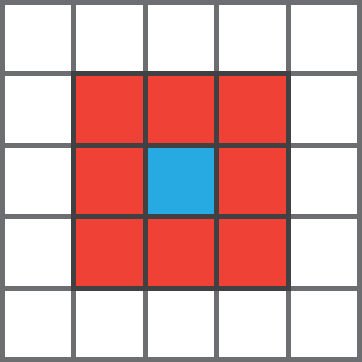
\includegraphics[width=\linewidth]{figures/moore}
    \caption{Moore neighborhood}
    \label{fig:moore}
  \end{subfigure}
  \begin{subfigure}[c]{.3\linewidth}
    \centering
    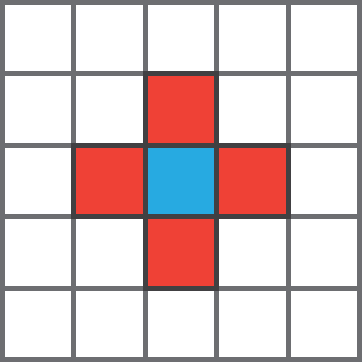
\includegraphics[width=\linewidth]{figures/von_neumann}
    \caption{Von Neumann neighborhood}
    \label{fig:von_neumann}
  \end{subfigure}

  \caption{Illustration of commonly used neighborhoods for 1D and 2D \ac{CA}.}
  \label{fig:neighborhoods}
\end{figure}

A \ac{CA} evolves in discrete time steps. An update rule
$\boldsymbol{\Phi}: \mathcal{S}^{s} \rightarrow \mathcal{S}$ defines the new state of a cell as a
function of its local neighborhood at the current time step. It is applied in
parallel to all the cells. For a \ac{CA} in its initial state at time
step 0 --- \ie a set of cells $\left(c_{i}^{(0)}\right)_{i \in \mathcal{L}} \in \mathcal{S}^{|\mathcal{L}|}$, and a
neighborhood function $\boldsymbol{N}$, we have the following update rule
\begin{equation}
\begin{aligned}
\forall i \in \mathcal{L}, \quad c_{i}^{(t + 1)} = \boldsymbol{\Phi}\left(\boldsymbol{N}\left(c_{i}^{(t)}\right)\right)
\end{aligned}
\end{equation}

The details of an example update step on a 1 dimensional \ac{CA} is shown on
Figure \ref{fig:ca_base}. The neighborhood of the cell $c_{i}$ is itself and the
two immediately adjacent cells.

\begin{figure}[htbp]
  \centering
 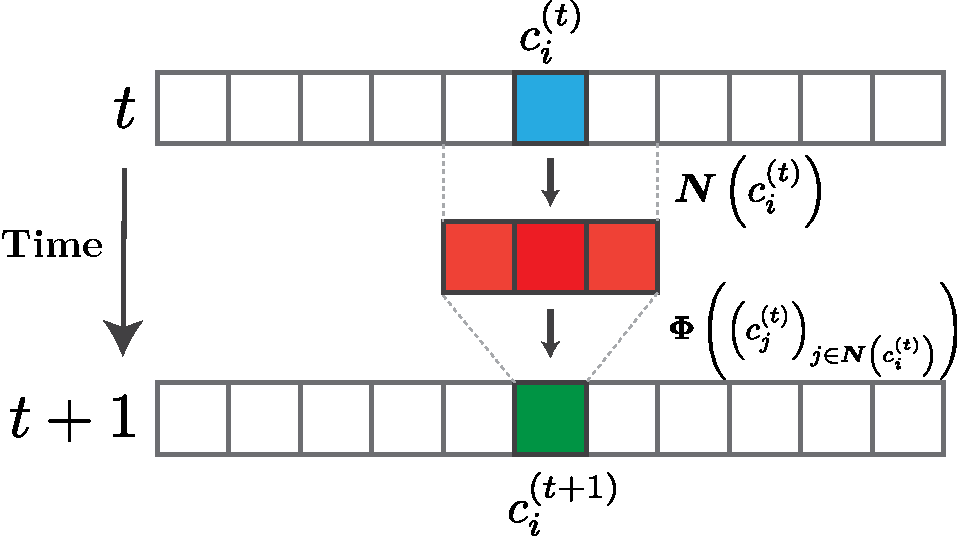
\includegraphics[width=.7\linewidth]{figures/ca_base}
  \caption{Illustration of a \acl{CA} update rule in 1 dimension. For each cell,
  we look up the neighboring cells and update its state according to the current
state of the neighbors.}
  \label{fig:ca_base}
\end{figure}

The function $\boldsymbol{\Phi}$ is often called a \emph{rule table} because it
associates an output state for each combinations of input neighbor states. These
output states can be looked up from a table containing all possible transitions
from inputs to outputs.

\paragraph{Rule representation}
A useful rule representation is obtained by listing all output state
corresponding to input configurations in a predetermined order. This results in
a list of values $[o_1, \ldots, o_{s^{|\mathcal{S}|}}]$, with $\forall i,\ o_{i} \in \mathcal{S}$, where $s$ is
the number of cells in a neighborhood, $\mathcal{S}$ is the space of available states and
$|\mathcal{S}|$ is the number of available states per cell. Using the $o_{i}$ as the
digits of a base-$|\mathcal{S}|$ number, each rule is uniquely represented by a number.
For example, as explained in more details in Section \ref{sec:elem-cell-autom},
the 256 binary rules in one dimension with neighborhood size 3 can be numbered from
0 to 255, and are referred to by their number in the literature.

\paragraph{Boundary conditions}
The grid of a \ac{CA} can be finite or infinite. In the infinite case, the grid
is assumed to be initialized to a uniform state except for a few cells set to
other states. The simulation is then run on these few cells while the rest of
the infinite grid does not have to be simulated from the start. For a finite
grid, an exhaustive simulation can be run, but there is a need to define
boundary conditions. The boundaries can be set to wrap to the other side of the
grid, forming a torus. An example of the corresponding indexing is given in
\eqref{eq:torus_index}. Other choices of boundary condition consists in adding
virtual padding cells outside of the main grid. They can be set to a fixed
state, a randomly chosen state, or mirror the cells on the inside of the grid.
Each of these choices affects the evolution and properties of the \ac{CA}, but
the importance of these boundaries decreases for very large grids.

\subsection{Classification of cellular automata\label{sec:class-cell-autom}}

Stephen Wolfram approached \acp{CA} as discrete, spatially extended dynamical
systems \parencite{wolframUniversalityComplexityCellular1984}. The analogy is
only superficial since many concepts from dynamical systems theory, such as
``chaos'', ``attractors'' and ``sensitivity to initial conditions'' only admit a
rigourous definition in the continuous state and continuous time models. Wolfram
proposed a qualitative classification of CA behavior roughly analogous to
classifications in dynamical systems theory, with four classes defined as
follows:

\begin{description}
  \item[Class 1] All initial configurations relax after a transient
        period to the same fixed configuration (e.g., all 1s).
  \item[Class 2] All initial configurations relax after a transient period to some
        fixed point or some temporally periodic cycle of configurations, but
        which one depends on the initial configuration. (\ac{CA} defined on
        finite lattices always end up having a periodic behavior because there
        is only a finite number of grid configurations. Class 2 does not refer to
        this type of periodic behavior but rather to cycles with periods much
        shorter than the total number of possible states).
  \item[Class 3] All initial configurations quickly exhibit chaotic behavior
        after a transient period. (The term “chaotic” here refers to
        apparently unpredictable space-time behavior.)
  \item[Class 4] Some initial configurations result in complex localized
        structures that can persist for a long time.
\end{description}

This classification being qualitative and not rigorous, there is not even a
clear consensus on which of the \acp{ECA} rules belong to class 4 or class 3.
Class 4 \ac{CA} rules are speculated to be capable of universal computation
\parencite{wolframUniversalityComplexityCellular1984}. For example,
\textcite{liStructureElementaryCellular1990} claimed that \ac{ECA} rule 110 has
class 4 behavior, and it was eventually proven to be universal
\parencite{cookUniversalityElementaryCellular2004}, but no other \ac{ECA} has
been proven universal since.

\textcite{zenilCompressionBasedInvestigationDynamical2010} studied the
compression size of the space-time diagrams of all \ac{ECA} for simulation of
fixed length. Using a simple k-means clustering technique, he obtained two
groups roughly matching Wolfram’s classes 1 and 2 and classes 3 and 4. We
reproduce these result on figure \ref{subfig:comp_scores}. This result offers an
interesting confirmation of Wolfram's classification that is not qualitative.
However, the results are very different if we modify the initial conditions as
well as the grid size, data representation, or compression algorithm
\parencite{hudcovaClassificationComplexSystems2020}.

\textcite{wuenscheGlobalDynamicsCellular1992} study the behavior of \acp{ECA}
when the simulations are reversed and computes the preimages of each
configuration. They introduce the Z-parameter which is the probability that a
partial preimage can be prolonged by one symbol for each \ac{CA}. He speculates
that class 4 occurs at $\text{Z} \approx 0.75$. This is not a classification,
but a class 4 membership test that can be computed from the rule directly,
making it practical compared to alternatives. In practice Wuensche's hypothesis
that $\text{Z} \approx 0.75$ corresponds to class 4 is rarely verified.

Hudcová defined a \ac{CA} classification that is based on the form of the
asymptotic growth of their transients, obtained through repeated simulation
\parencite{hudcovaClassificationComplexSystems2020,
  hudcovaClassificationDiscreteDynamical2022}.

\subsection{Cellular automata variants}

A large number of variants of \acp{CA} have been proposed, modifying or
constraining various part of the definition above. We list some common ones
here.

\paragraph{Elementary cellular automata.\label{sec:elem-cell-autom}}
\Acp{ECA} are the 1 dimensional \acp{CA} with two states per cell and
neighborhood size 3 --- the cell and its two direct neighbors on the 1D grid.
There are 8 possible configurations of a neighborhood with 3 cells and 2 states
per cell, which corresponds to 256 possible ways to define an \ac{ECA} --- two
possible outputs for each of these 8 possible configurations, hence
$2^{8} = 256$ possible \ac{CA}. This relatively small number of rules enables
exhaustively exploring the rule space and mapping out the \ac{ECA} properties,
which would not be possible for general \acp{CA}.

\begin{figure}[htbp]
  \centering
  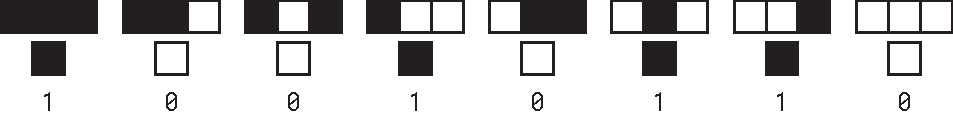
\includegraphics[width=.95\linewidth]{figures/eca_150_rule}
  \caption{Illustration of the rule of \ac{ECA} number 150.}
  \label{fig:eca_150_rule}
\end{figure}

These \acp{CA} are studied extensively, and offer an interesting combination of
trivial definition and implementation and complex and unpredictable properties.
One fundamental problem of \ac{CA} research is to classify the 256 rules into
well-defined behavior types and order them by complexity, which was attempted in
several previous works \parencite{wuenscheGlobalDynamicsCellular1992,
  gutowitzTransientsCyclesComplexity1991,
  wuenscheClassifyingCellularAutomata1999, wolframNewKindScience2002,
  zenilCompressionBasedInvestigationDynamical2010,
  hudcovaClassificationComplexSystems2020,
  hudcovaComputationalHierarchyElementary2021}. We discuss these classifications
in more details in section \ref{sec:class-cell-autom}.

\begin{figure}[htbp]
  \centering
\begin{subfigure}[b]{.45\linewidth}
  \centering
  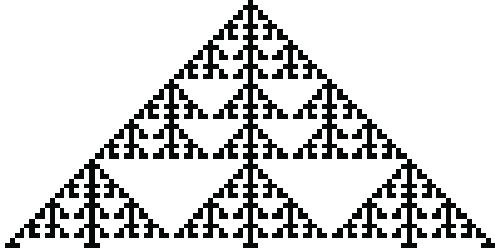
\includegraphics[width=\linewidth]{figures/eca_150_single.pdf}
  \caption{Single cell initialization}
  \label{fig:eca_150_single}
\end{subfigure}
\begin{subfigure}[b]{.45\linewidth}
  \centering
  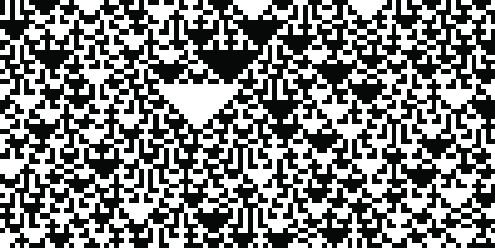
\includegraphics[width=\linewidth]{figures/eca_150_random.pdf}
  \caption{Random initialization}
  \label{fig:eca_150_random}
\end{subfigure}
\caption{Evolution of \ac{ECA} number 150 simulated on a grid of size 100 for 50
  steps. \ref{fig:eca_150_single} shows a simulation starting from a blank grid
  with only one cell set to 1. \ref{fig:eca_150_random} shows a simulation
  starting from a random initialization.}
  \label{fig:eca_150}
\end{figure}


\ac{ECA} rules are easily visualized, because there are only 8 possible
neighborhood configurations that need to be shown. For example, figure
\ref{fig:eca_150_rule} shows the transition table for \ac{ECA} rule 150. If we
assign 1 to the black state and 0 to the white state, the possible neighborhood
configurations are ordered in their binary order from right to left, with the
leftmost bit being the most significant one. This is how the rule number is
computed, using the output states (last row on figure \ref{fig:eca_150_rule}) as
a binary representation.

\paragraph{Totalistic cellular automata.}
Totalistic \ac{CA} are a subset of \ac{CA} which rules can be expressed as a
function of the sum of neighboring cell values. These \ac{CA} were introduced by
Stephen Wolfram \parencite{wolframStatisticalMechanicsCellular1983}. For
example, \ac{ECA} 150 which rule is shown on figure \ref{fig:eca_150_rule} is a
totalistic \ac{CA}. Its rule could be summarized as ``if exactly two states are
1 or all states are 0, the next state is 0, otherwise if one or three states are
1, the next state is 1''. Conway's Game of Life, presented below, is an example
of totalistic \ac{CA} in two dimensions.

\paragraph{Game of Life.\label{sec:game-life}}
The game of life is one of the most famous \ac{CA}. It was proposed by
mathematician John Conway in 1970 \parencite{gardnerMathematicalGames1970}. It
is a two dimensional binary \ac{CA}. Its two states are often called ``alive''
and ``dead''. Its rule can be summarized in three sentences as follows.
\begin{itemize}
  \item Any live cell with two or three live neighbours survives.
  \item Any dead cell with three live neighbours becomes a live cell.
  \item Other live cells and already dead cells die in the next generation.
\end{itemize}
This \ac{CA} has a particularly active community dedicated to finding
interesting patterns with particular properties such as a period length or speed
of movement through the grid. Some of these patterns have been used as memory
registers and communication channels to build a Universal Computer
\parencite{IgblanLifeUniversal}. This construction proves that the game of life
is Turing-complete. This property is thought to be also shared by other \ac{CA}
--- it is proven for at least \ac{ECA} rule 110
\parencite{cookUniversalityElementaryCellular2004}. This makes \ac{CA} models
theoretically appealing for the design of a learning algorithm because they can
simulate any algorithm.

\begin{figure}[htbp]
  \centering
  \begin{subfigure}[t]{.31\linewidth}
    \centering
    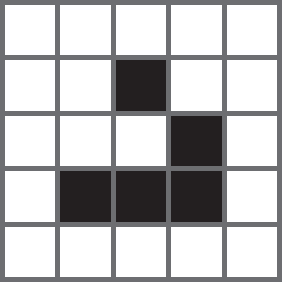
\includegraphics[width=\linewidth]{figures/glider.pdf}
    \caption{Moving oscillator (\emph{glider}).}
    \label{fig:glider}
  \end{subfigure}
  \begin{subfigure}[t]{.31\linewidth}
    \centering
    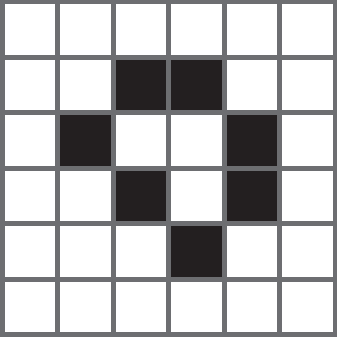
\includegraphics[width=\linewidth]{figures/still_life.pdf}
    \caption{Fixed pattern (\emph{still life}).}
    \label{fig:still_life}
  \end{subfigure}
  \begin{subfigure}[t]{.31\linewidth}
    \centering
    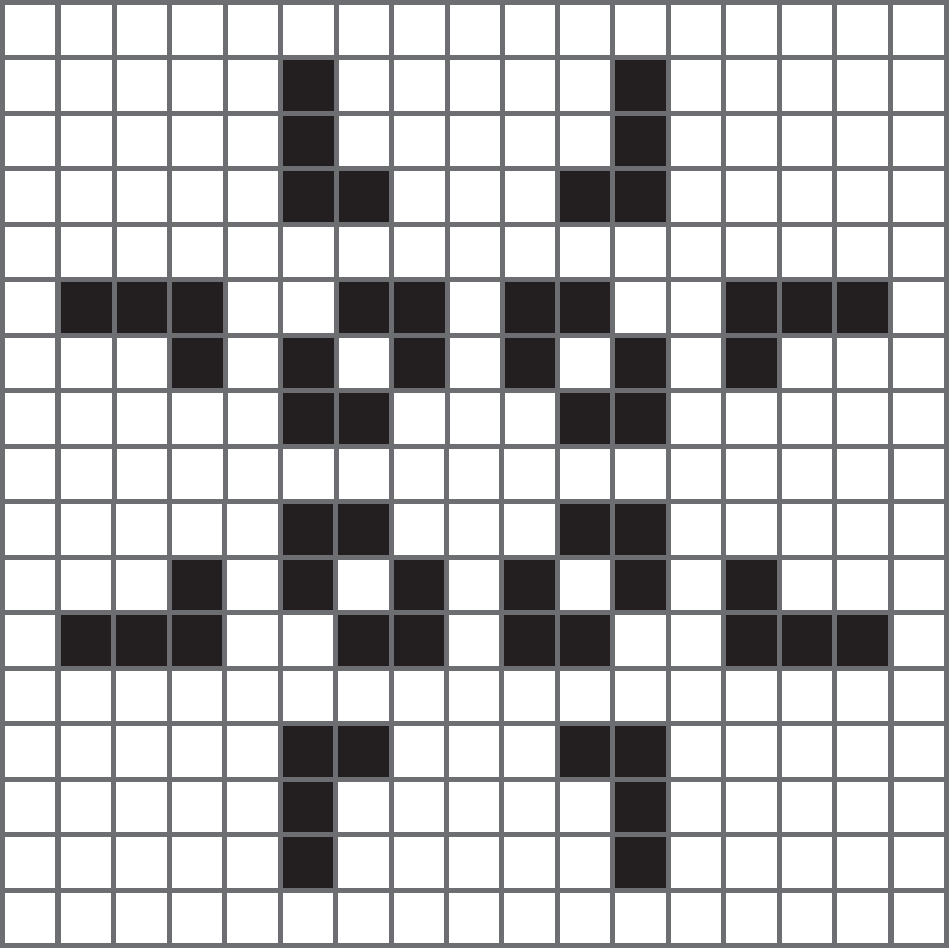
\includegraphics[width=\linewidth]{figures/pulsar.pdf}
    \caption{Period 3 oscillator (\emph{pulsar}).}
    \label{fig:pulsar}
  \end{subfigure}

  \caption{Some game of life patterns with various properties. The moving
    oscillator \ref{fig:glider} moves 1 cell along the bottom right diagonal
    every 4 steps. The fixed pattern \ref{fig:still_life} never changes except
    if it interacts with others. The oscillator \ref{fig:pulsar} loops through
    three different configurations.}
  \label{fig:gol_patterns}
\end{figure}


\paragraph{Asynchronous cellular automata}
A cellular automaton is said to be asynchronous when its cells are not all
updated in parallel at each time step. Several cell update schemes can
be chosen. Contrary to regular cellular automata, the grid has to be finite
for an update rule to exist. This is because asynchronous \ac{CA} have to define
an order of update of the cells which would not be defined on an infinite grid.
This update order can be random, follow a predefined order or be decided by a
global controller. Groups of cells can be updated simultaneously or updates can
be done cell by cell. The many effects of the asynchronous updates can be hard
to predict and make these type of \ac{CA}

Asynchronous \ac{CA} are an appealing model when using large systems for which
parallel update is prohibitively expensive. The rule could adapt itself and
preferentially update cells form active or useful parts of the \ac{CA} while
doing slower updates to the less active parts of the \ac{CA}. An asynchronous
\ac{CA} with evolutionary properties was constructed in
\parencite{nehanivEvolutionAsynchronousCellular2003}. The authors argue that
asynchronicity is a strong advantage for constructing systems that can evolve
within \acp{CA}.

\paragraph{Stochastic cellular automata}
In a stochastic cellular automaton, the update function $\boldsymbol{\Phi}$ is
stochastic. This means that the next state of all the cells of the grid is
sampled from a probability distribution that depends on the current neighborhood
configuration. We can write
\begin{equation}
\begin{aligned}
  \forall i \in \mathcal{L},\ s \in \mathcal{S} \quad p\left(c_{i}^{(t + 1)} = s \right) = \boldsymbol{\Phi} \left(\boldsymbol{N}\left(c_{i}^{(t)}\right)\right)(s).
\end{aligned}
\end{equation}
These \ac{CA} have interesting applications in physics
\parencite{vichniacSimulatingPhysicsCellular1984,
  ottaviSimulationIsingModel1989} or biology
\parencite{boasCellularPottsModel2018}.

\paragraph{Continuous}
Another family of \ac{CA} uses real-valued states, often restricted to the
range $[0, 1]$. The update function is then a real multivariate function
\begin{equation}
  \begin{aligned}
  \boldsymbol{\Phi}: [0, 1]^{s} \rightarrow [0, 1].
  \end{aligned}
  \label{eq:phi_cont}
\end{equation}

Examples of continuous \ac{CA} include Lenia
\parencite{chanLeniaBiologyArtificial2019a}, or \acp{NCA}
\parencite{mordvintsevGrowingNeuralCellular2020}.
\textcite{garzonRealComputationCellular1993} explores the condition for a
real-valued \ac{CA} to be able to compute real-valued functions.

\paragraph{Higher dimensional cellular automata}
\acp{CA} of dimension higher than 2 have been comparatively less studied for
several reasons, including the limits that arise when simulating and visualizing
systems in more than 2 dimensions on a computer screen. Another problem is with
the exploding number of possible rules in higher dimensions. The number of
neighbors per cell grows exponentially with the dimension, and the number of
possible rules has a doubly exponential rate of growth. This makes the
convenient representation of \acp{CA} rules as tables infeasible, since the size
of that table quickly exceeds the available memory of most computers. For
example, there are $2^{512} \approx 10^{154}$ possible 2D rules with 2 states and a
Moore neighborhood, which is already an incomprehensibly large number, but there
are $2^{134,217,728} \approx 10^{40,403,562}$ such rules in 3D.

Despite these limitation several works have studied higher dimensional \acp{CA},
although mostly in 3 dimensions
\parencite{tsalidesThreedimensionalCellularAutomata1989,
  sudhakaranGrowing3DArtefacts2021}. For example, there are several examples of
successful 3D \acp{CA} simulations applied to material sciences
\parencite{gandin3DCellularAutomaton1997, arataFreeformShapeModeling1999,
  panStudyFailureScale2009, dicaprio3DCellularAutomata2016}.

\paragraph{Hexagonal cellular automata}
Hexagonal cellular automata are defined on grids tiled with hexagons, where each
cell has 6 direct neighbors.

\begin{figure}[htbp]
  \centering
  \begin{subfigure}[b]{.35\linewidth}
    \centering
    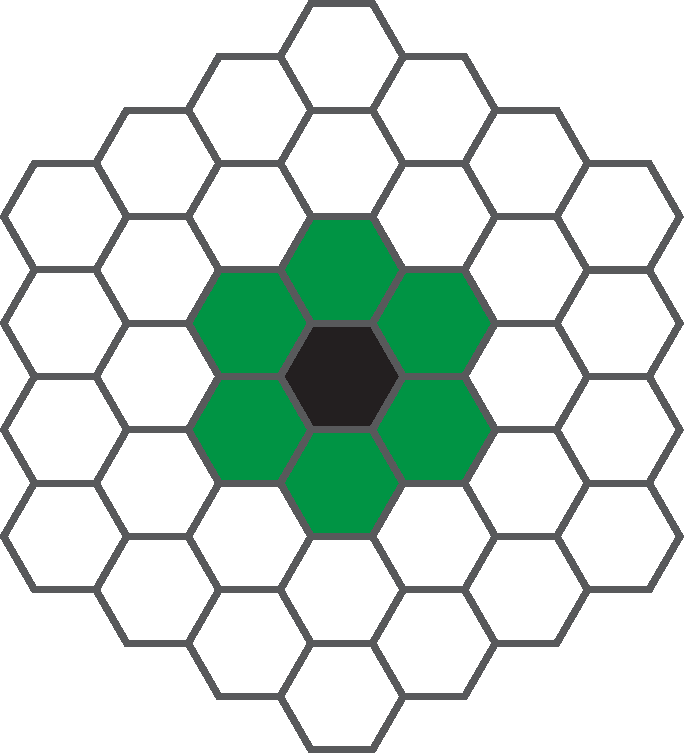
\includegraphics[width=\linewidth]{figures/hexagonal_1}
    \caption{Range 1 neighborhood}
    \label{fig:hexagonal_1}
  \end{subfigure}
  \hspace{10pt}
  \begin{subfigure}[b]{.35\linewidth}
    \centering
    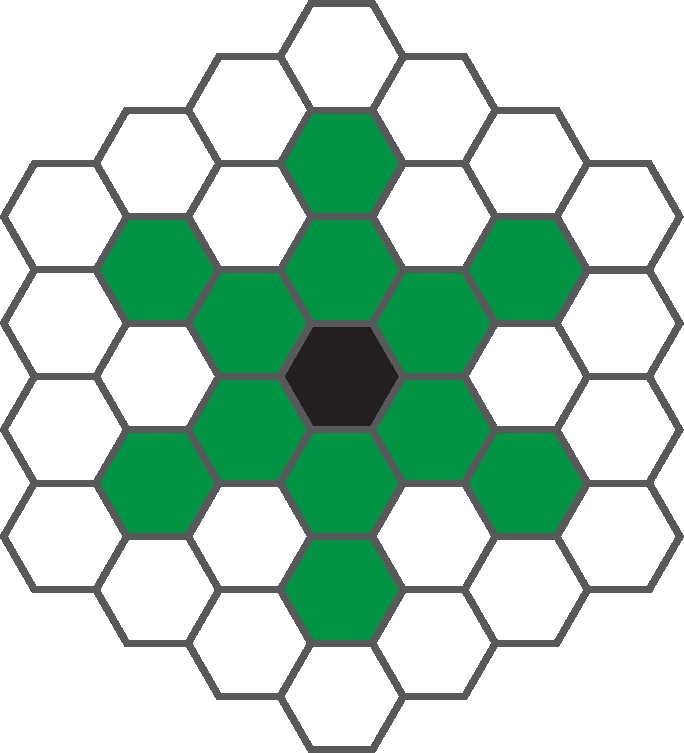
\includegraphics[width=\linewidth]{figures/hexagonal_2}
    \caption{Ray neighborhood}
    \label{fig:hexagonal_2}
  \end{subfigure}
  \caption{Example definition of neighborhood for hexagonal cellular automata.}
\label{fig:hexagonal}
\end{figure}


\subsection{Parametrizing and sampling CA rules}
As explained in \ref{sec:challenges}, one of the main challenges of working with
complex systems is the parametrization and control of the behavior of that
system. \ac{CA} are no exception, and several parametrization schemes have been
proposed, having their respective benefits and drawbacks. There are infinitely
many ways to define rules for \acp{CA}, and for each of these definition a very
large number of rules is available, making it impossible to sample a significant
portion of the rule space. A good parametrization allows scanning a wide range
of behavior of \ac{CA} by traversing the space in an interesting way.

\paragraph{Langton's lambda\label{sec:langtons-lambda}}

Christopher Langton proposed one of the first parameter that could be used to
control the behavior of \acp{CA} to some extent
\parencite{langtonStudyingArtificialLife1986, langtonComputationEdgeChaos1990}.
For a \ac{CA} with $K = |\mathcal{S}|$ states, and a state arbitrarily chosen to be
the \emph{quiescent} state (this corresponds to the ``dead'' state in the game
of life for example), if there are $n$ transitions to the quiescent state within
the rule table and $K^{s} - n$ remaining transitions that do not lead to the
quiescent state, where $s$ is the number of cells in the neighborhood, we
have

\begin{equation}
  \label{eq:langton}
  \begin{aligned}
    \lambda = \frac{K^{s} - n}{K^{n}}.
  \end{aligned}
\end{equation}

For Langton, the purpose of $\lambda$ is to search the space of \ac{CA} in an ordered
manner by varying the value of the parameter. His procedure starts with a rule
with all transitions leading to the quiescent state. The value of $\lambda$ is
increased in discrete steps up to $1 - 1 / K^{n}$ by randomly changing
transitions of the rule to lead to a different state. An illustration of the
behavior change of a \ac{CA} rule under this procedure is shown on figure
\ref{fig:langton_lambda}. Langton collects various measures of the dynamical
behavior of \ac{CA} and studies them as a function of $\lambda$. He observes a phase
transition as $\lambda$ approaches its maximal value where the \acp{CA} seem to behave
in the most complex way, with long transients and large scale propagating
structures. He calls this phase transition ``edge of chaos'' because it
corresponds to $lambda$ values just before the generated \acp{CA} become
chaotic.

\begin{figure}[htbp]
  \centering
  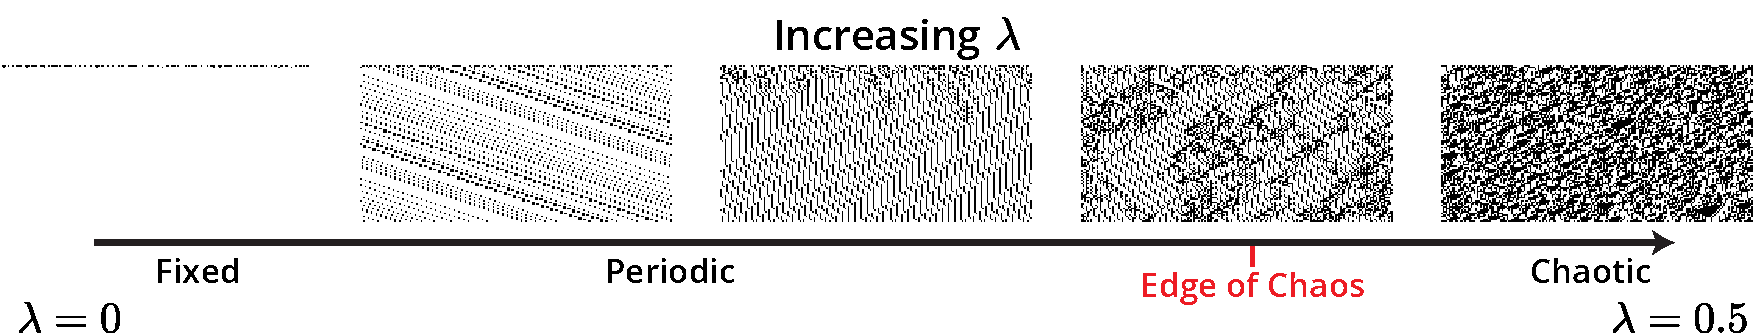
\includegraphics[width=\linewidth]{figures/langton_lambda.pdf}
  \caption{The effect of varying $\lambda$ for a 1D binary \ac{CA} rule. A \ac{CA}
    rule is progressively modified along a trajectory of increasing $\lambda$. The
    rule starts with a fixed behavior, becomes periodic and then complex when
    hitting the ``edge of chaos''. Note the localized structures that spread
    over time (down along the y axis) and interact in the fourth figure. When
    $\lambda$ increases further the rule becomes chaotic.}
  \label{fig:langton_lambda}
\end{figure}

\paragraph{Dirichlet sampling}
For an arbitrary number of states and neighborhood size, it can be challenging
to sample \ac{CA} while scanning a wide range of behavior. This is because the
size of the space of \acp{CA} rules is very large. The naive method of uniformly
sampling each transition output is not useful in large rule spaces with multiple
states, large neighborhoods or grid dimension higher than 1.

Rules with equal proportions of transitions leading to all states tend to be the
most chaotic. This is also what Langton observed when studying the $\lambda$
parameter. This is explained by the fact that sampling each transition output
uniformly is equivalent to sampling the rules from a multinomial distribution
with the number of possible states ($K$), number of possible transitions
($n = K^{K^{s}}$, with $s$ the number of cells in a neighborhood) and uniform
probabilities $p_{1}= \ldots= p_{K}$ as parameters. A random variable
$X = (X_{1}, \ldots, X_{K})$ indicates the number of times each outcome is observed.
The probability mass function of this distribution is

\begin{equation}
  \label{eq:multinomial}
  \begin{aligned}
    P(X_{1}=x_{1}, \ldots , X_{K}=x_{k}) = \frac{n!}{x_{1}!\cdots x_{K}!} p_{1}^{x_{1}}\cdots p_{K}^{x_{K}}.
  \end{aligned}
\end{equation}

This quantity gets small for large $n$ and rules with output transition skewed
towards a specific state. For example, the binary game of life rule has 372
transitions that lead to the state 0 and 140 that lead to the state 1. The
probability of sampling a rule with these transition proportions is
$8.24\mathrm{e}{-26}$, making it very unlikely to obtain such a rule with a
uniform transition sampling method.

We propose Dirichlet sampling as an alternative way to sample rules with fixed
ratio of transitions leading to output states. For a rule with $K$ states, we
sample a $K$-uple from a Dirichlet distribution of order $K$ with parameters
$(\alpha_{k})_{k\in [1, K]}$ where $\alpha_{0} = \alpha_{1} = \ldots = \alpha_{K} = \alpha < 1$. The result is a
quantile $K$-uple $(q_{1}, \ldots, q_{K})$. For $\alpha < 1$, the distribution is
concentrated around the corners of a simplex of dimension $K$.

Rules are sampled so that the number of transition to each output state matches
the quantile generated from the Dirichlet distribution. Samples will be more
likely to have a dominant quantile which can be associated with the quiescent
state in Langton's $\lambda$ calculation. The resulting sampling of cellular automata
is much better for scanning the whole space of rules and generating \ac{CA}
rules which would be unreachable with the naive sampling method, as illustrated
on figure \ref{fig:ca_rule_sampling}.

\begin{figure}[htbp]
  \centering
  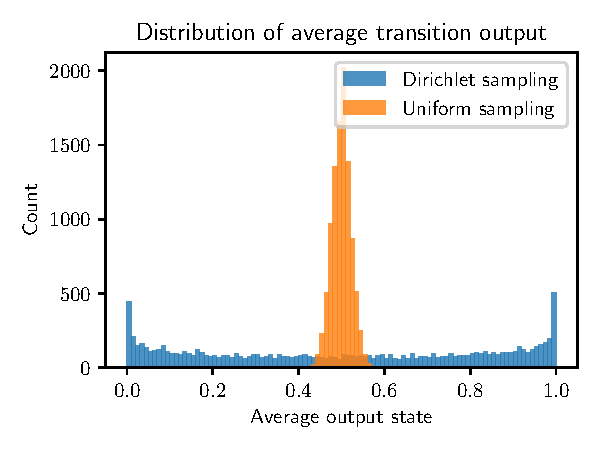
\includegraphics[width=.5\linewidth]{figures/ca_rule_sampling_hist}
  \caption{An illustration of the difference between naive uniform rule sampling
    and Dirichlet sampling on binary rules. 10000 2D binary CA rules were
    sampled with each method, the plot displays an histogram of their average
    output state. Uniform sampling leads to more rules with an average output
    state close to 0.5, meaning approximately as many transitions towards both
    states. Dirichlet sampling can control, through the choice of parameter $\alpha$,
    how much rules with more skewed transitions should be sampled which is
    visible with the spiked on the blue histogram close to 0 and 1.}
  \label{fig:ca_rule_sampling}
\end{figure}

\paragraph{Smooth sampling with the recurrent convolutional neural network
  analogy}


\section{Cellular automata and RNNs}\label{sec:cell-autom-rnns}
The purpose of this section is to show that cellular automata and recurrent
convolutional neural networks have very strong connections and to draw this
parallel as clearly as possible. We express the \ac{CA} update function as a set
of convolutional operations that can be derived from any \ac{CA} rule.

This connection yields interesting consequences both for the theoretical
properties of these models and the potential applications of cellular automata
and recurrent networks. It shows for instance that emergent properties with
increasing complexity and perhaps open-ended development are possible within the
hidden state of a recurrent neural network.

The conceptual similarity between \acp{CA} and neural networks comes to no
surprise. Fundamentally, \ac{CA} represent the paradigm of emergence, whereby
the origins of complex behaviors are searched for in an assemblage of possibly
very simple parts rather than viewed as a sum of complex building blocks. It is
often argued that there is no better known example of a truly emergent
phenomenon than that of the emergence of consciousness out of the large network
of functionally simple (and certainly unconscious) neuronal components that make
up the human brain. A biological neural network, like a \ac{CA}, consists of a
large space of interconnected nodes, with a dynamical behavior that is a local
function of other nodes to which it is connected. Artificial neural networks can
be thought of as being a set of biologically inspired CA rules
\parencite{ilachinskiCellularAutomataDiscrete2001}. The more precise parallel
between cellular automata and a form of recurrent/convolutional network has also
been drawn by several other researchers
\parencite{wulffLearningCellularAutomaton1993,
  gilpinCellularAutomataConvolutional2018,
  mordvintsevGrowingNeuralCellular2020}.

\begin{figure}[htbp]
  \centering
  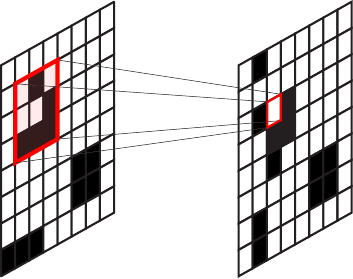
\includegraphics[width=.3\linewidth]{figures/ca_cnn}
  \caption{\label{fig:ca_cnn}The CA update rule is local and can be represented
    by a convolutional neural networks: linear local uniform transformations
    followed by the application of a non-linear function.}
\end{figure}

\subsection{RNN formalism}

\begin{figure*}[!ht]
  \centering
  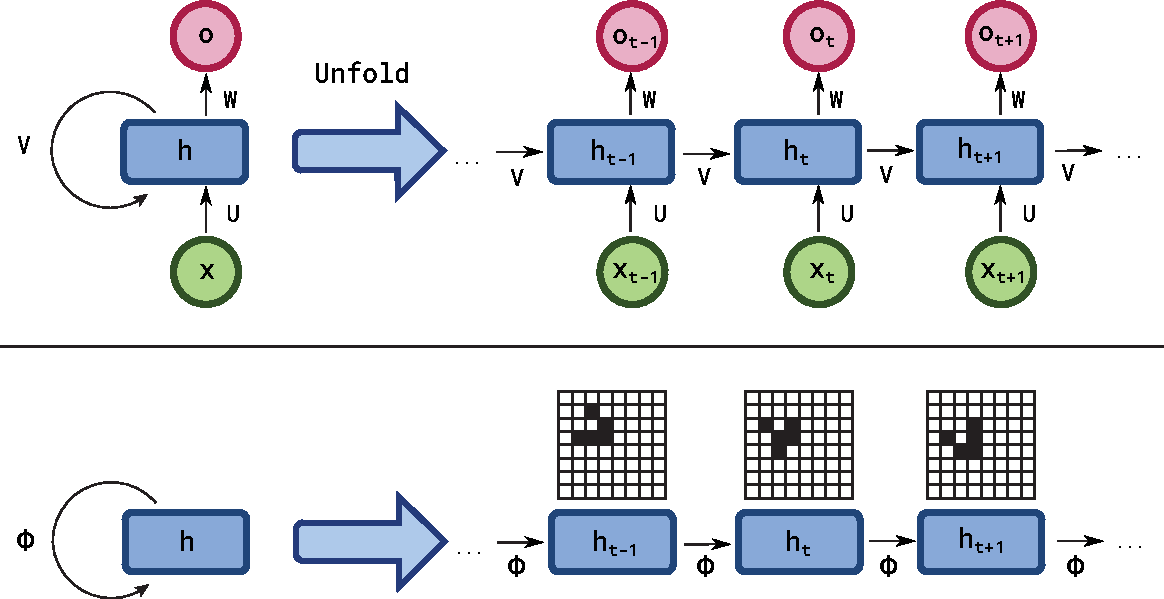
\includegraphics[width=\linewidth]{figures/rnn_and_gol.pdf}
  \caption{\label{fig:standard_rnn} Standard RNN architecture (left) and Game of
    Life seen as a RNN with no inputs and outputs (right). For the \ac{CA}, the
    ``hidden'' state $h_t$ is the current state of the grid at timestep $t$. The
    operator $\boldsymbol{\Phi}$ is the \ac{CA} update rule which is
    equivalent to a \ac{CNN} (see Section~\ref{sec:transition-rule-as}). This
    illustration is based on
    \href{https://commons.wikimedia.org/wiki/File:Recurrent_neural_network_unfold.svg}{Recurrent
      neural network unfold} by
    \href{https://commons.wikimedia.org/wiki/User:Ixnay}{fdeloche}, licensed
    under \href{https://creativecommons.org/licenses/by-sa/4.0/}{CC BY 4.0}.}
\end{figure*}


We write the definition of a cellular automaton with RNN-inspired formalism and
notations. This parallel is illustrated on Figure~\ref{fig:standard_rnn}.

The grid state at time $t$ is denoted $h_t$ and corresponds to the hidden state
in a RNN\@. In the case of classical CAs, it is a 1 or 2D vector of discrete
values, but~\parencite{mordvintsevGrowingNeuralCellular2020} and other CA
extensions use continuous values, much like the usual RNNs.

The transformation $\Phi$ operates on this hidden state only. It is equivalent
to a convolutional layer as explained below in
Section~\ref{sec:transition-rule-as}.

Inputs and outputs $(\mathbf{x}, \mathbf{o})$ are not included in the classical
definition of CAs but are an easily implementable extension as discussed in
Section~\ref{sec:adding-inputs-outp}.

\subsection{Transition rule as a set of convolutions\label{sec:transition-rule-as}}

Each cell $c_i$ from the above definition is represented as a vector of size $k$
the number of states. Cell $c_i$ is in state $s_i \in [0, \ldots, k - 1]$. A
neighborhood of size $3$ in a $1$D CA ($r=1$) is a $3 \times k$ vector
$\mathbf{u}_i = [u_{i-1}, u_{i}, u_{i+1}]$. Each $u_{ij}$ is a vector of size
$k$ with a $1$ in position $s_i$. This is illustrated in the 1D (resp.\ 2D) case
on the left (resp.\ right) of Figure~\ref{fig:cell}. For a CA with only two
states, it is redundant to have a $3\times 2$ vector, but this ``one-hot'' encoding
becomes helpful when working with more states.

\begin{figure}[htbp]
  \centering
  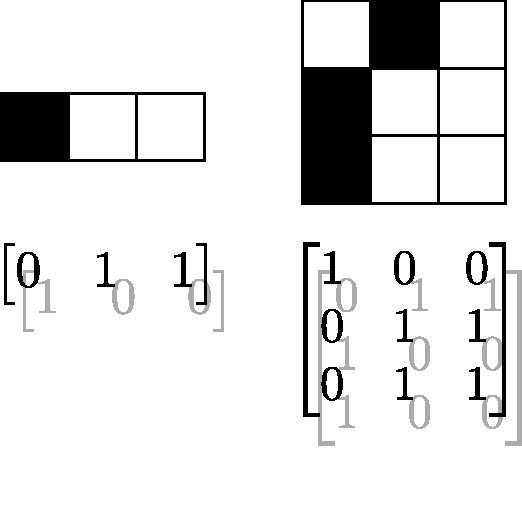
\includegraphics[width=.3\linewidth]{figures/repr}
  \caption{\label{fig:cell}Cellular automaton neighborood vector representation
    example with 2 states. A $3\times 3$ square of cells with two states can be
    represented by a $3\times 3 \times 2$ vector. Left: 1D 3-neighbors
    representation. Right: 2D $3\times3$ neighbors representation.}

\end{figure}

\begin{figure}[htbp]
  \centering
  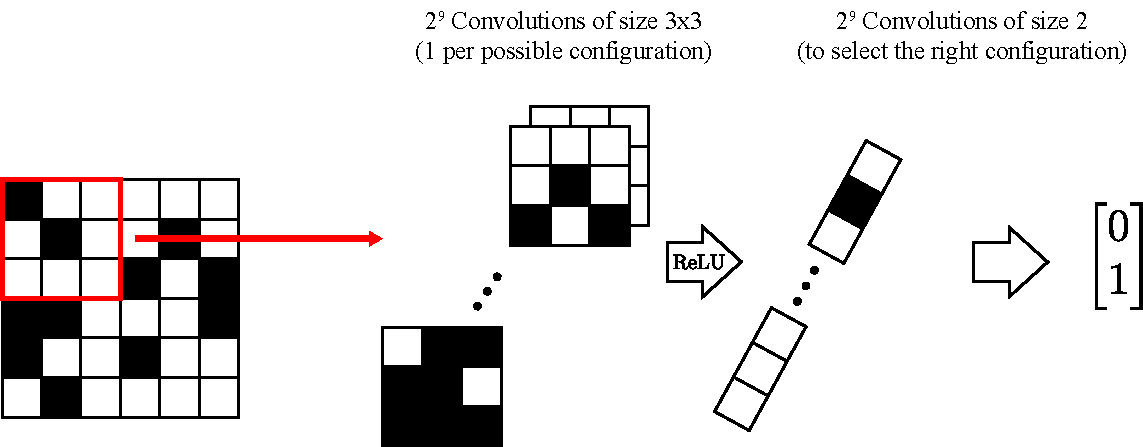
\includegraphics[width=.9\linewidth]{figures/global_schema}
  \caption{\label{fig:global_schema}How to represent any 2-states 2D CA rule
    operating on $3\times 3$ neighborhoods as a 2 layers CNN.}
\end{figure}


With this representation, on can easily express the transition rule $\Phi$ as a
simple convolutional neural network. This network would be composed of 2 layers
which are shown on Figure~\ref{fig:global_schema}:

\paragraph{The first convolutional layer}It is receptive to each possible
neighborhood configuration. This layer is composed of $k^{2r + 1}$ filters of
dimension $k\times (2r + 1)$ with only ones and zeros, that are each the same as
a possible configuration of size $(2r+1)$ of the neighborhood. The product of
each filter with an input neighborhood will be an integer between $0$ and $9$.
By applying a ReLU non-linearity with a vector of 8s as bias, we obtain the
input to the second layer, a vector of size $k^{2r + 1}$ for each cell with
plays the role of an indicator of the input configuration.

\paragraph{A second convolutional layer} It has $k^{2r + 1}$ filters of size $1$ that
are either $0$ or $1$ depending on the desired output of the transition.

\subsubsection{Recurrent convolutions in machine learning}

Recurrent convolutional networks have been used in several areas of machine
learning such as NLP or computer vision
\parencite{pinheiroRecurrentConvolutionalNeural2014,
  laiRecurrentConvolutionalNeural2015}.

\subsection{Adding inputs and outputs\label{sec:adding-inputs-outp}}

Figure~\ref{fig:standard_rnn} shows clearly where the ``missing'' inputs and
outputs could be added in Game of Life or any other CA\@. We can think of many
possible forms.

\subsubsection{Inputs}
There are many ways to add inputs to the model presented above. We divide our
proposed methods into two classes: inputs that directly modify the hidden state
during the CA evolution and inputs that augment the hidden state and affect the
rule.

\begin{description}

\item[Hidden state augmentation and rule modulation]
Inputs are usually added to the hidden state just before the application of the
non-linearity in standard RNNs.

In the case of cellular automata, it can also be done in the following ways:

\begin{figure*}[ht]
  \centering
  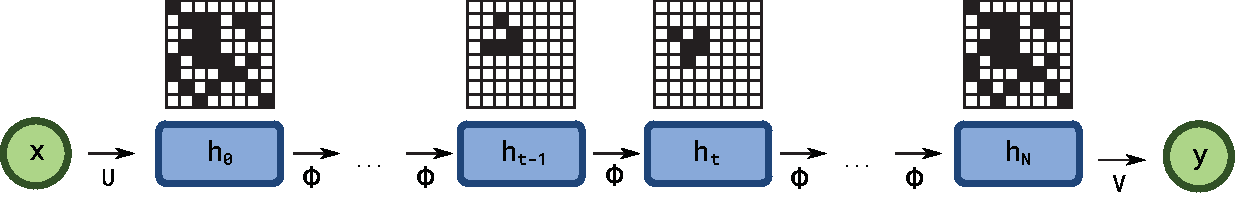
\includegraphics[width=.9\linewidth]{figures/encode_decode.pdf}
  \caption{\label{fig:encode_decode} Inputs and outputs can be directly
    encoded within the hidden state.}
\end{figure*}

\item[Vector state] A simple to add inputs to a cellular automaton is to
consider the grid as having an additional (possibly read-only) dimension. For
example, a 1D automaton would actually be represented by a vector with dimension
$N\times 2$ where the first vector of size $N$ is the grid state and the other
is the input. The update rule would be changed so as to add this new component
into account. One can see this model as using multiple CA rules at the same
time, with the input state conditioning the rule being chosen for a given update
step.

\item[Variable update rule] Inputs can also influence a CA's evolution by
changing the update rule. With this configuration, the update rule $\Phi$ is now
a function of the input $x$. We now have $\Phi_x = G(x)$, where

\[G: \mathcal{X} \rightarrow \left({\{ 1, \ldots, k \}}^{2r+1} \to \{1, \ldots, k\}\right)\]


A similar approach was used in \parencite{adamsFormalDefinitionsUnbounded2017}. It
showed that conditioning a CA update rule on another CA's evolution could enable
a higher diversity of behavior.

\item[Concatenation] Input can be concatenated to the hidden state (\eg~on
the grid boundaries) before applying the update rule, forming a sort of fixed
read-only memory space. Concatenation is illustrated in Figure~\ref{fig:concat}.
A possible disadvantage of this method is the fact that information need to
propagate through the grid if it is to be processed far from where the read-only
memory was positioned.

This approach is more computer-like, reserving some space for different
functionalities of the data.

\begin{figure}[ht]
  \centering
  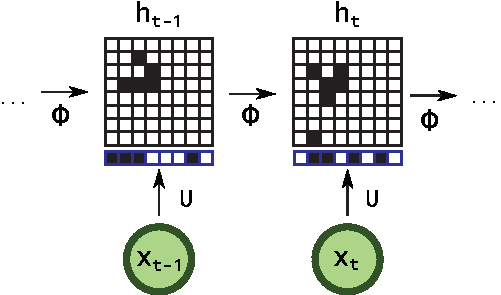
\includegraphics[width=.5\linewidth]{figures/concat.pdf}
  \caption{\label{fig:concat} Input $x_t$ is projected and concatenated to
    hidden state $h_t$, affecting the boundary conditions of the cellular
    automaton.}
\end{figure}

\item[Hidden state manipulation]

Another approach is to directly modify the hidden state to ``communicate''
information to the system. These methods are used
in~\parencite{mordvintsevGrowingNeuralCellular2020,
  randazzoSelfclassifyingMNISTDigits2020} to make interactive demos and allow
users to directly modify that hidden state. A user can interact with the
system by drawing with its mouse. This sets parts of the internal state to a
fixed cell state.

\item[Masking] Input data can serve as a mask on top of the current grid
state, forcing some cells into states that depend on the input values. If we
view the state activations in the CA as some neural pattern, this approch can
be seen as a form of \emph{neuromodulation}, which has previously been used in
machine learning \parencite{soltoggioEvolutionaryAdvantagesNeuromodulated2008,
  ishiguroNeuromodulatedControlBipedal2003,
  beaulieuLearningContinuallyLearn2020}.

A mask can be constructed from an input
vector $x$ by linearly transforming $x$ and applying an activation function
(\eg~step function). It controls which channels are activated, and where
information can flow or not. This kind of mask can be applied with element-wise
multiplication or addition but also more elaborate operations. It is illustrated
in Figure~\ref{fig:mask}.

\begin{figure}[ht]
  \centering
  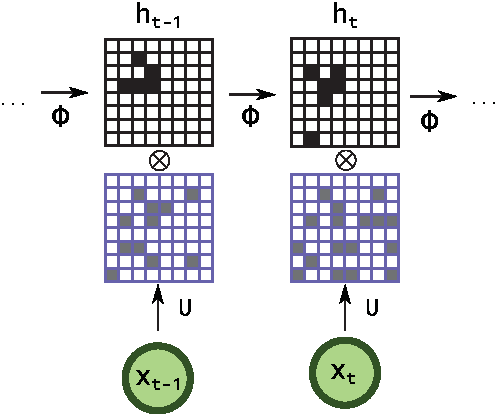
\includegraphics[width=.5\linewidth]{figures/mask.pdf}
  \caption{\label{fig:mask} Input is converted into a mask for the hidden state.
  The mask is applied through element-wise multiplication here.}
\end{figure}

\end{description}

\subsubsection{Outputs}

Similarly, inputs can be extracted from the hidden state in several different
ways. One might read outputs from the boundaries of the grid, from a
transformation of the grid using a neural network, etc. The output could also be
stored within an additional dimension of the ``extended'' grid state presented
above.

\subsubsection{Cellular automata and computations}

From a computational point of view, the hidden state can be seen as a working
tape that some kind of \emph{parallel Turing machine} (the cellular automaton)
is doing computation on. In this framework, the input is encoded as the initial
state of the tape and decoded from the last state of the tape (as illustrated on
Figure~\ref{fig:encode_decode}). The recurrent convolutional neural network
(RCNN) then plays the role of a fixed computer program. This is the setting
adopted in previous works on constructing computations with cellular automata: a
task is chosen, and one searches for rules which can execute that task on
input/output pairs~\parencite{mitchellComputationCellularAutomata2005}. Previous
successes with RNNs demonstrate that this model is powerful enough to learn
complex functions when the grid is made of continuous numbers and the
transformation is not local thanks to optimization, for instance in language
modelling.

However, this gets more interesting when we consider the input as encoding both
some data and a computer program, as it is the case with a Turing machine. We can
then expect a cellular automaton (or RNN) to not only compute the result of a particular
function, but to be equivalent to a general purpose computer capable of
computing the result of any chosen algorithm without any need for optimization.


\subsection{Consequences}

Viewing cellular automata as a recurrent convolutional neural networks  as
described above has several interesting consequences.

\subsubsection{Turing-completeness of the system}

Because we can simulate rule 110 ECA in the above system, it follows from the
Turing-completeness of this CA rule that the above system is Turing-complete.
This is a interesting result, albeit not very significant since RNN have already
been proven to be
Turing-complete~\parencite{siegelmannComputationalPowerNeural1992}, with very
little practical implications. The model is in practice relatively far from a
real world CNN with a fixed number of layers independent from one another ---
compared to a variable number of steps and shared layers for the
automaton-RCNN\@.

\subsubsection{Differentiable cellular automata}

Every step of the computations involved in computing a step of a cellular
automaton represented as a RCNN is differentiable. We can therefore
theoretically couple this framework with backpropagation to make
\emph{learnable} cellular automata that can adapt their rules to minimize a
target loss function.

This is the direction taken by~\textcite{mordvintsevGrowingNeuralCellular2020}.
The authors use supervised learning on a cellular automaton and train it to get
a stable self-repairing target shape.

However, because supervised cellular automata can only do as much as they have
been trained to do, I believe it defeats the purpose of working with a model
capable of spontaneous complex emergent behavior. Open-ended complexity increase
could very unlikely be achieved through pure supervision.

\textcite{gilpinCellularAutomataConvolutional2018} takes the reverse approach, and
tries to train RCNNs to simulate a fixed CA rule, using the training process as
a way to help understand the structure of CA rule space.

\subsection{Beyond the naive rule representation}

The above representation of cellular automata rules is a one-to-one mapping.
Each automata rule has its CNN counterpart and vice versa. However, there are
more efficient ways to represent CA rules. For instance, we can make the first
layer of filters receptive both to a given configuration and its inverse
(\eg~$(1, 0, 1)$ and $(0, 1, 0)$ in a ECA) by using negative values in the
filter (use a filter $(1, -1, 1)$ instead of $(1, 0, 1)$ and $(0, 1, 0)$
separately).

For example, game of life doesn't need more than 2 convolutional filters or
parameters to be represented by a CNN because it is totalistic (a cell's new
state only depends on the number of neighbors in state 1 and its current state).


\section{Reservoir computing \label{sec:res-models}}
\Ac{RC} is a computational framework that aims to exploit the states of a
complex dynamical system to perform some target task
\parencite{tanakaRecentAdvancesPhysical2019}. It relies on a \emph{reservoir} of
computations, that is a dynamical system performing operations on its internal
state. An input signal is fed into this reservoir, that behaves as a black box
from the point of view of the algorithm. Input values can be sequential or
non-sequential. They are projected and combined with the dynamical system using
a suitable mechanism. This projection can be learned, set randomly, or chosen.
The internal state of the dynamical system evolves according to the its update
rule. Finally the a decoder model (usually a linear regression), is trained in a
supervised manner to extract necessary information from the internal state of
the dynamical systems to predict the right output. A general diagram describing
this process is displayed on figure \ref{fig:reservoir_diagram}.

\begin{figure}[htbp]
  \centering
  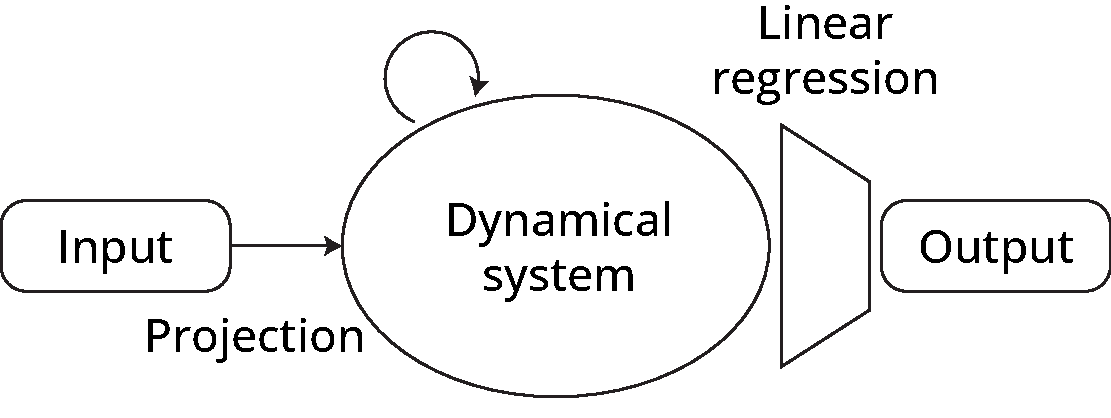
\includegraphics[width=.8\linewidth]{figures/reservoir_schema}
  \caption{Diagram of the general functioning of a \ac{RC} system. Input values
    are projected in the state or evolution function of a dynamical system which
    is run according to its internal rule. Output values are decoded from the
    internal state of the dynamical systems with a trainable layer.}
  \label{fig:reservoir_diagram}
\end{figure}

Some early known formulation of \ac{RC} are due to
\textcite{kirbyContextDynamicsNeural1991}. Another early formulation of the idea
was done by \textcite{schomakerNeuralNetworkModels1990,
  schomakerSimulationRecognitionHandwriting1991,
  schomakerNeuralOscillatornetworkModel1992}.

In another early work, \textcite{buonomanoTemporalInformationTransformed1995}
used a random spiking neural network with excitatory and inhibitory elements.
Neuron connection probabilities were inspired by real rat brain data
\parencite{masonSynapticTransmissionIndividual1991}. He observed a interval
sensitive response of these neurons when subjected to pulses spaced by varying
time intervals. This indicates an ability to encode temporal information. To
measure this phenomenon he trained an output linear layer to recognize specific
patterns in the activation of the last layer of neurons. This idea of using a
randomly initialized neural network with fixed weights and train a simple linear
layer to decode outputs was reinvented later under the names ``Echo-state
networks'' \parencite{jaegerEchoStateApproach2001} and ``Liquid state machines''
\parencite{maassRealTimeComputingStable2002}.

Another advantage of reservoir computing is that, because the reservoir can be
implemented using a variety of physical systems, substrates, and devices. These
type of reservoirs are sometimes called ``exotic''
\parencite{lukoseviciusReservoirComputingApproaches2009}, but physical \ac{RC}
shows promises to develop cheap and efficient machine learning hardware and can
inform us on the nature and behavior of the underlying physical systems.
\textcite{tanakaRecentAdvancesPhysical2019} lists several types of \ac{RC}

\begin{description}
  \item[Dynamical systems] The \ac{RC} models based on other reservoirs than
        random \acp{RNN}. This includes reservoir computing with \aclp{CA},
        which we give more detail about in section \ref{sec:app-ca-res}.
  \item[Electronic \ac{RC}] These models are implemented on electronic circuits,
        such as artificial neural networks implemented on physical circuits or
        other neuromorphic circuits. For example, \ac{RC} models can be build on
        FPGAs \parencite{antonikApplicationFPGAReal2018,
        verstraetenReservoirComputingStochastic2005,
        alomarLowcostHardwareImplementation2014,
        antonikFPGAImplementationReservoir2015} or memristive circuits
        \parencite{yangInvestigationsStaircaseMemristor2016,
        merkelMemristiveReservoirComputing2014,
        donahueDesignAnalysisNeuromemristive2015}.
  \item[Photonic \ac{RC}] The principle of photonic \ac{RC} is to use optical
        reservoirs to generate the computations. A first example using
        semiconductor optical amplifiers (SOAs) was proposed by
        Vandoorne and colleague \parencite{vandoorneOpticalSignalProcessing2008,
        vandoorneParallelReservoirComputing2011} and subsequently built \parencite{vandoorneExperimentalDemonstrationReservoir2014}.
        Other works use that scattering of light in complex media
        \parencite{dongOpticalReservoirComputing2020,
        rafayelyanLargeScaleOpticalReservoir2020}.
  \item[Spintronic \ac{RC}] Some \ac{RC} works used nanosacle electronics
        involving the charge and spin of electrons called \emph{spintronics}
        \parencite{wolfSpintronicsSpinBasedElectronics2001}. Spintronics have
        been used in multiple ways to build \ac{RC} models, using spin torque
        oscillators (STO)
        \parencite{torrejonNeuromorphicComputingNanoscale2017,
        williameChaoticDynamicsMacrospin2019}, or spin waves
        \parencite{nakaneReservoirComputingSpin2018}.
  \item[Mechanical \ac{RC}] Soft mechanical bodies have complex nonlinear
        dynamics that can be beneficial to build a \ac{RC} model
        \parencite{pfeiferHowBodyShapes2007}. For example, a reservoir using a
        mass-spring network was proposed by
        \textcite{hauserTheoreticalFoundationMorphological2011}.
  \item[Biological \ac{RC}] There have been multiple hypotheses on whether the
        parts of the brain behaves like a \ac{RC} system
        \parencite{yamazakiCerebellumLiquidState2007}. For example, a \ac{RC}
        model was proposed to understand the mechanism of context-dependent eye
        movement \parencite{domineyComplexSensorymotorSequence1995,
        domineyModelCorticostriatalPlasticity1995}.
\end{description}

\subsection{Reservoir computing applications}

\subsection{Echo-state network}

The \acf{ESN} (and simultaneously developed model \emph{Liquid state machine}
(LSM)) is the most well known implementation of the \ac{RC} principle
\parencite{tanakaRecentAdvancesPhysical2019}. The main idea behind this model is
to drive a \ac{RNN} with some input signal, which will excite the neurons within
the reservoir and induce several non-linear response signals. This is combined
with a trainable linear regression to extract a desired output from a
combination of these response signals.

In practice, the input projection is often fixed but it can also be trainable.
The output can also be fed back to the reservoir like an input, and the
structure of the \ac{RNN} reservoir can be adapted.

\begin{figure}[htbp]
  \centering
  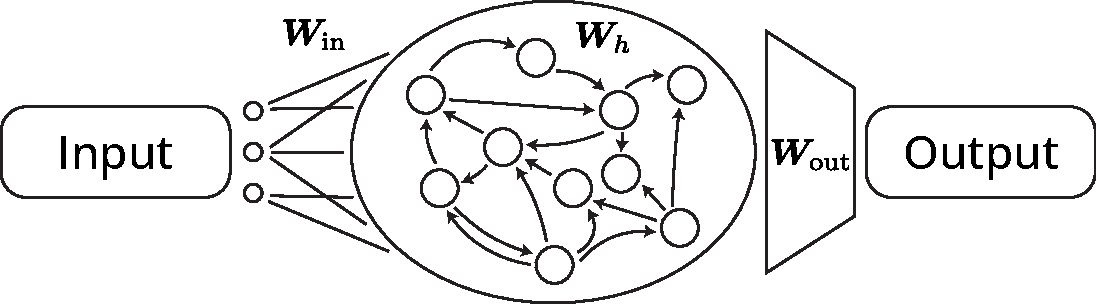
\includegraphics[width=.8\linewidth]{figures/echo_state_network}
  \caption{Diagram of an echo-state network. The \ac{RNN} is reprensented
    ``flattened'' in time. The circles represent the units of the hidden state
    of the \ac{RNN}. An arrow between unit $i$ and $j$ corresponds to a non-zero
    entry in the matrix, $\mW_{h, ij} \neq 0$. Non-linear operations are not
    represented.}
  \label{fig:echo_state_network}
\end{figure}

We define an input sequence to be $(\vx_{t})_{t=1}^{T}$. The initial state of
the reservoir at $t = 0$ is $\vr_{0}$. The echo-state network is based on the
following update equation:
\begin{equation}
  \label{eq:esn}
  \vr_{t + 1} = (1 - \alpha) \vr_{t}
  +
  \beta \tanh(\mW_{h}\: \vr_{t} + \mW_{\text{in}}\: \vx_{t + 1}),
\end{equation}
where $\vr_{t}$ is the $K$-dimensional state vector -- corresponding to the
hidden neurons --- at time $t$, $\beta$ is the leaking rate,
$\mW_{h} \in \mathbb{R}^{K \times K}$ is a sparsely connected random hidden
layer matrix, and $\mW_{\text{in}} \in \mathbb{R}^{L \times K}$ is the input
projection matrix. The matrices $\mW_{h}$ and $\mW_{\text{in}}$ are set to
random values.

For the random initialization of $\mW_{h}$ and $\mW_{\text{in}}$
\textcite{jaegerLongShortTermMemory2012} recommends: $\mW_{h}$ should have an
average of 10 non-zeros entries per row, all sampled uniformly in $[-1, 1]$.
Then the matrix is scaled to attain a set spectral radius $\rho$ which is
optimized for each experiment in \parencite{jaegerLongShortTermMemory2012}.
$\mW_{\text{in}}$ has its entries uniformly sampled in $[-1, 1]$. Then columns
of the matrix are individually scaled with factors
$\sigma_{1}, \ldots, \sigma_{L}$ specific to each experiments. In this
formulation, there are multiple parameters to optimize:

\begin{itemize}
  \item The reservoir size $K$
  \item The spectral radius of $\mW_{h}$, $\rho$
  \item The input weights scaling parameters $\sigma_{1}, \ldots, \sigma_{L}$
  \item The leaking rate $\beta$
\end{itemize}

\textcite{jaegerLongShortTermMemory2012} explores three
optimization schemes for these parameters:
\begin{description}
  \item[Blind] The input weights scaling parameters are all set to a single
        value $\sigma$. The parameters $K$, $\rho$, $\sigma$ and $\beta$ are
        optimized. This corresponds to a search space of dimension 4.
  \item[Basic] Each of the $\sigma_{i}$ are optimized individually, or in
        groups. The other parameters are also optimized.
  \item[Smart] All the parameters are optimized like in the \textbf{Basic}
        scheme, and the weights of $\mW_{h}$ are also crafted specifically for
        the target task.
\end{description}


The $L$-dimensional outputs are computed at times $t > 0$ as
\begin{equation}
  \label{eq:esn-res}
\tilde{\vx}_{t+ 1} = D(\vr_{t}),
\end{equation}
where $D: \mathbb{R}^{K} \rightarrow \mathbb{R}^{L}$ is a (trained) decoding
function. For echo-state networks, the decoder is often a linear transformation
$D(\vr_{t}) = \mW_{\text{out}} \vr_{t}$ where $\mW_{\text{out}}$ is a
$K \times L$-dimensional matrix. In our experiments, we set $\beta = 0$, which
was empirically observed to yield the best results on our tasks. The parameter
$\beta$, as well as the randomly sampled weight matrix, are sometimes tuned for
each task \parencite{jaegerLongShortTermMemory2012}. We only use default values
to get a task-independent setup with the least possible assumptions and to make
the methods comparable.

\subsection{Reservoir cellular automata\label{sec:app-ca-res}}

Cellular automata can be used as the dynamical system in reservoir computing.
This was originally proposed by Yilmaz in 2014 and later named ReCA (Reservoir
Cellular Automata) \autocite{yilmazReservoirComputingUsing2014,
  margemExperimentalStudyCellular2017}.

Several implementations of ReCA systems have been proposed and evaluated on
various tasks \autocite{yilmazReservoirComputingUsing2014,
  nicheleDeepLearningCellular2017, nicheleDeepReservoirComputing2017,
  nicheleReservoirComputingUsing2017, margemReservoirComputingBased2018,
  kleykoCellularAutomataCan2020, babsonReservoirComputingComplex2019,
  ,mcdonaldReservoirComputingExtreme2017a}. In this section we lay out a general
description of reservoir computing with cellular automata based on these
previous works and present our proposed extensions.

\paragraph{Encoding\label{sec:encoding}}
Input data is assumed to be categorical and sequential,

\[
  X = [X_{1}, \ldots, X_{t}, \ldots],\quad t\in \mathbb{N}, \quad \forall t \ X_{t} \in \mathcal{X} \subset \mathbb{N}.
\]

A cellular automaton is a discrete system which is not particularly designed to
handle inputs. The purpose of the encoding step in ReCA is to convert the input
data points to vectors that can be embedded in the cellular automaton state
space. Such encoding should translate --- or embed --- the input space
$\mathcal{X}$ to a new one that can be combined with the current state of the
cellular automaton. The goal is to make a cellular automaton ``react'' to its
input and leverage the resulting computation to solve a problem.

\paragraph{Input projection}

First, each categorical input vector is one-hot encoded into a vector of size
$L_{in}$, where $L_{in} = |\mathcal{X}|$ is the number of input categories. We have
\[\forall t,\quad \mathbf{x}_{t} \in {\{0, 1\}}^{L_{in}},\] with
$\sum_{i = 1}^{L_{in}}{(\mathbf{x}_{t})}_{i} = 1$.

Next, the vectors $\mathbf{x}_{t}$ are projected to vectors
$\mathbf{p}_{t} = P(\mathbf{x}_{t}) \in \mathcal{P} = {\{0, 1\}}^{L_{d}}$ of
fixed size $L_{d}$. Usually we have $L_{d} > L_{in}$, . In our work we compute
this projection in one of three ways:

\begin{description}
  \item[One-to-one] each input bit is mapped to a single index in $\mathbf{p}$.
        This is the projection function first proposed in
        \textcite{yilmazReservoirComputingUsing2014}.
\end{description}

We also propose two novel projection schemes and compare them to the previous
ones. They extend the one-to-one projection and allow for a richer variety of
produced encodings:

\begin{description}
  \item[One-to-many] each input bit is mapped to exactly $k$ positions in $P$
        instead of one. This is equivalent to adding $k$ separate and mutually
        exclusive one-to-one projections into a single one.
  \item[One-to-pattern] each input bit is mapped to a random contiguous pattern
        of $k$ bits set to a fixed position.
\end{description}

The effect of applying our three methods on a simple input with three components
is illustrated in Fig.~\ref{fig:enc_meth}. Projections are chosen so as to make
each input bit map to a unique output configuration.

\begin{figure}[htbp]
  \centering
  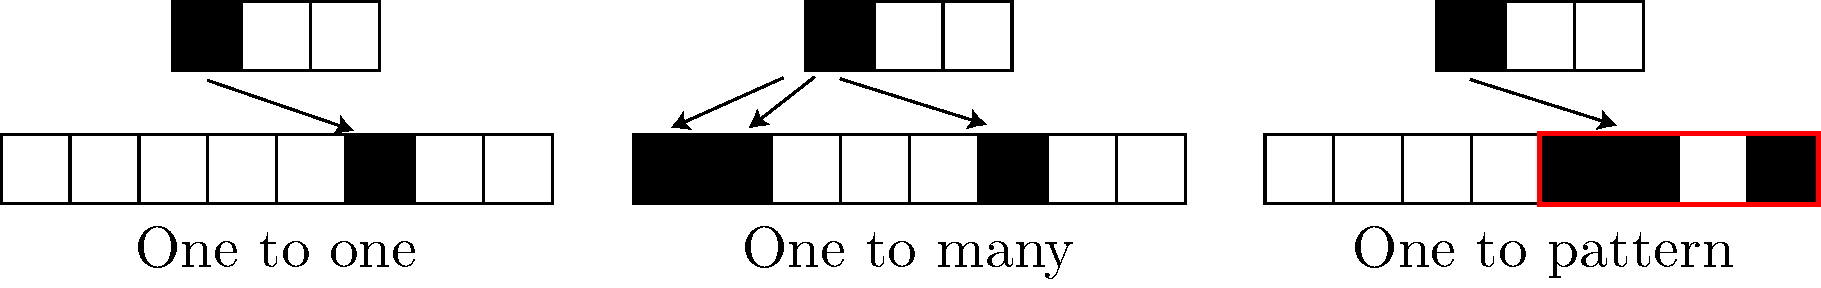
\includegraphics[width=\linewidth]{figures/encoding_methods.pdf}
  \caption{Three encoding methods. From left to right: \emph{one-to-one},
    \emph{one-to-many} and \emph{one-to-pattern}.}\label{fig:enc_meth}
\end{figure}

Following \parencite{yilmazReservoirComputingUsing2014,
  nicheleReservoirComputingUsing2017, nicheleDeepLearningCellular2017}, the
input is projected multiple times to add redundancy to the encoding. This was
experimentally observed to improve performance. We also use a projection vector
larger than the initial one. The projections are randomly generated $R$ times,
applied and concatenated as a single large encoder to create the full CA input
vector. The parameter $R$ is called \emph{redundancy}.

For cellular automata in 1D, the space $\mathcal{P}$ is one-dimensional and the
concatenation is simply done over this dimension. In higher dimensional spaces,
this concatenation has to be defined in some other way.

We write the $R$ projection functions $E_{1}, E_{2}, \ldots, E_{R}$. The
final size of the input vector and the CA state grid is $R \times L_{d}$. We have
\begin{align}
  \vp_{t} = E_{1}(\vx_{t})\mathbin\Vert \ldots \mathbin \Vert E_{R}(\vx_{t})
\end{align}
where $\mathbin\Vert$ is the concatenation operator.

Other projections have been proposed and implemented, for example in
\parencite{yilmazReservoirComputingUsing2014}. We choose to present the three
above because they are simple to understand and implement and their effects can
be explored thoroughly.

\paragraph{Input combination}
There are multiple ways to combine the input vector with the current \ac{CA}
state. \textcite{gloverDynamicalLandscapeReservoir2021} propose to use a XOR
function between the projected input and the \ac{CA} state.

At each input step $t$, the projected input vector $\vp_{t}$ is XORed
element-wise with the current CA state $\vs_{t}$, so that each 1 bit from the
input switches the corresponding bit in the CA state to another value. This
creates a new state $\vs_{t}'$ that the CA will evolve from. $\vs_{t}'$ is
defined as
\begin{align}
  \vs_{t}' \coloneqq \vp_{t} \otimes \vs_{t},
\end{align}
where $\otimes$ is the element-wise XOR operator between two vectors of binary
values, and $\vs'_{t}$ is the temporary CA state resulting from the combination
of the CA state and input vectors at time $t$.

From the \ac{CA} state $\vs'_{t}$, We then compute the next CA states by
applying the update function $\Phi$,

\begin{equation}
  \label{eq:ca-state}
  \vs_{t + 1} = \Phi(\vs'_{t}).
\end{equation}

This is one of many possible ways to combine an input vector with the current
state of the CA that may affect its performance as a reservoir. The XOR-based
input combination gives asymmetrical role to 0 and 1 in the input vectors, which
is natural considering the way we encode and project the categorical data
points. Different cellular automata rules might benefit or get lower performance
because of these encoding choices. The combination problem can be generalized to
incorporate it to the \ac{CA} rule search problem. We demonstrate this in the
next paragraph.

\paragraph{Generalization.} We generalize the input combination method above by
incorporating it to the \ac{CA} update rule. Since the input vector $\vp$ is
binary, we may treat its value at position $i$ as just another virtual \ac{CA}
cell. For an standard \ac{ECA}, the update step takes into account the three
immediate neighbors $\vs^{(i - 1)}, \vs^{(i)}, \vs^{(i + 1)}$ plus the additional
virtual cell $\vp^{(i)}$. Instead of 8 possible input configuration, we now have
16. In this extended \ac{CA} space, the number of possible rules is
$2^{16} = 65536$ instead of 256.

\begin{figure}[htbp]
  \centering
    \begin{subfigure}[b]{.387\linewidth}
    \centering
    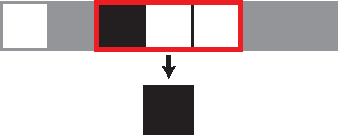
\includegraphics[width=\linewidth]{figures/ca_update_rule.pdf}
    \caption{Regular CA update only takes neighbor states into
      account.}\label{fig:standard-ca-update}
  \end{subfigure}
  \hspace{10pt}
  \begin{subfigure}[b]{.55\linewidth}
    \centering
    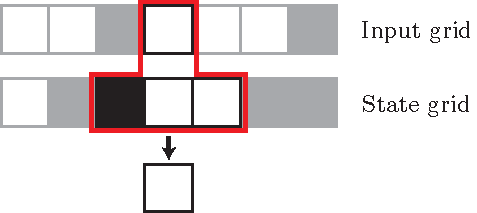
\includegraphics[width=\linewidth]{figures/generalized_ca_update_rule.pdf}
    \caption{The extended neighborhood update also uses an input value to
      decide the next state of a cell.}\label{fig:generalized-ca-update}
  \end{subfigure}
  \caption{Comparison of standard CA update rule and our extended input
    combination rule.\label{fig:ca_update_rule}}
\end{figure}

This method is illustrated in Fig.~\ref{fig:ca_update_rule} along the regular CA
update. It generalizes the concept of input combination with the state $\vs$.
The XOR method described above is one of its special cases, but our method also
contains all the possible boolean function with 4 inputs.

\paragraph{Building the reservoir}
The final reservoir state $\vr_{t + 1}$ is obtained by concatenating $r$
consecutive CA states obtained from a single combined state $\vs'$ by applying
$\Phi$ again. If the size of the state is $n$, the resulting reservoir vector
$\vr$ has a dimension $K = r \times n$, where $r$ is defined above. As for the
\ac{ESN}, the $L$-dimensional output tokens are calculated at times $t > 0$ as
$\tilde{\vx}_{t+ 1} = D(\vr_{t})$ where
$D: \mathbb{R}^{K} \rightarrow \mathbb{R}^{L}$ is the (trained) decoding
function. Usually a linear decoding function is used, such that
$D(\vr_{t}) = \mW_{\text{out}}\vr_{t}$. The complete process of \ac{RC} with
\ac{CA} is summarized in figure \ref{fig:reca-schema}.

\begin{figure}[htbp]
  \centering
  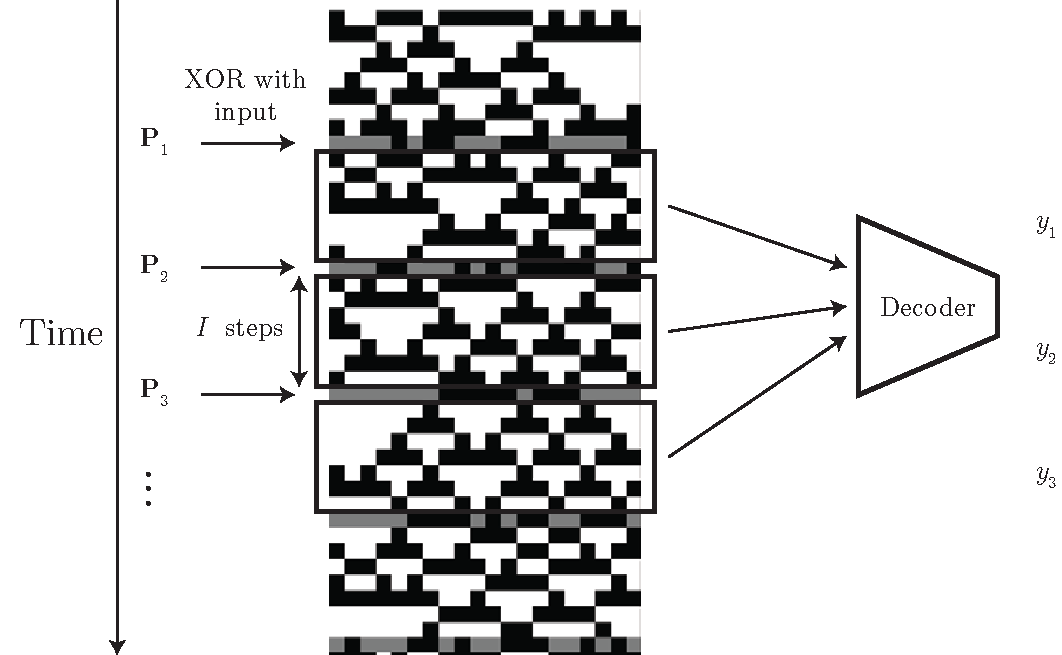
\includegraphics[width=.6\linewidth]{figures/reca_schema.pdf}
  \caption{Global illustration of the ReCA model with the usual XOR-based
    combination.}\label{fig:reca-schema}
\end{figure}

\section{Measuring complexity}

Measuring the complexity of a system is a fundamentally difficult task. Many
complex systems exhibit what Peter Grassberger calls \emph{self-generated
  complexity} \parencite{grassbergerQuantitativeTheorySelfgenerated1986}. This
means that the formulation of the problem is translationally invariant and the
observed structure arises from a spontaneous breakdown of translational
invariance. Unfortunately there is no universally accepted and formalized notion
of ``complexity'', even though most intuitively agree that it exists. No clear
observable and protocol have been proposed that would give a quantitative notion
of complexity. \textcite{grassbergerProblemsQuantifyingSelfgenerated1989} argued
that no single quantity is sufficient to measure complexity, since it depends on
how meaning is assigned to this term. Even when meaning has been fixed by the
definition of an observable quantity, the statistics of the measurement of this
observable are crucial to its interpretation
\parencite{gutowitzCellularAutomataSciences1995}.


\subsection{Information based measures}

We note that one of the most widely known concept of complexity of symbol
sequences, the ``algorithmic complexity'', should rather be called a measure of
information. In the literature, measures of information are commonly used as
complexity metrics. These quantities are better measures of ``randomness'' than
complexity, but they are nonetheless important for the study of complex systems.

\subsubsection{Information content}
For an event $E$ with probability $P$, the information content of this event is
defined as the negative logarithm of its probability, that is

\begin{equation}
  I(E) :=  -\log(P).
\end{equation}

This metric quantifies how unlikely an event is and depends on how the
probability $P$ was estimated in practice. This notion is at the foundation of
information theory.

\subsubsection{Shannon Entropy}
Shannon entropy is defined as the expected information content of the input
\parencite{shannonMathematicalTheoryCommunication1975}. We have

\begin{align*}
  H(X) := \mathbb{E}[-\log(P(X))].
\end{align*}

This measure is a lower bound on the number of bits the input could be
compressed down to.

In the case of a 1D \ac{ECA}, the Shannon entropy could be computed cell-wise
over the time distribution of the states. Yielding an entropy per cell score
that can be averaged over a entire automaton. This measure is for instance one
of the measures used by Wolfram in
\parencite{wolframStatisticalMechanicsCellular1983} and by Langton in
\parencite{langtonComputationEdgeChaos1990} to study how the parameter $\lambda$
affects the behavior of the automaton. There are several ways to compute it when
dealing with a CA, depending on what part of the CA is considered as the main
random variable. If the CA is finite, the state at timestep $t$ can be seen as a
random variable that can take one of $2^N$ possible values (with $N$ the width
of the automaton state). In that case, the probability of a state can easily be
estimated by counting its number of occurrences during evolution.

\subsubsection{Rényi Entropy}
The Rényi entropy is a generalization of Shannon entropy that gives different
weights to events of various probabilities. It is formally defined for an
$\alpha \geq 0, \alpha \neq 1$ and $X$ random variable with possible outcomes
$0, 1, ..., n$ as
\begin{align*}
  H_\alpha(X) = \frac{1}{1-\alpha} \log\left(\sum_{i=0}^np_i^\alpha\right)
\end{align*}

In the limit $\alpha \rightarrow 1$ it is equal to the Shannon entropy, where
each events probabilities are equally important. $\alpha \rightarrow \infty$
yields the Min-entropy, and we have $H_{\infty} (X) = \min_{i}(\log(p_{i}))$.
With $\alpha \rightarrow 0$ Rényi entropy is the same as Max-entropy. Rényi
entropy was used by \textcite{wolframStatisticalMechanicsCellular1983} to
estimate entropy in infinite CAs.

\paragraph{Mutual information}
The mutual information is a measure of the dependence between two variables. Two
independent variables will have a mutual information of zero. If the two are
strongly dependent, for example if one is a function of another, the mutual
information between them will be large.

\textcite{chaitinMathematicalDefinitionLife1987} proposes to split a system into
blocks of fixed sizes and calculate the mutual information among its components.
He uses the maximum value of the mutual information in all possible partitions
define "life" in a mathematical way. \textcite{shawDrippingFaucetModel1984} and
\textcite{grassbergerQuantitativeTheorySelfgenerated1986} also use the mutual
information measure between two semi-infinite blocks in a sequence to define
complexity. Mutual information is also used to study the complexity of cellular
automata as the parameter $\lambda$ is changed (for details about the $\lambda$
in the context of \ac{CA}, see section \ref{sec:langtons-lambda})
\parencite{gutowitzMethodsDesigningCellular1988,
  liTransitionPhenomenaCellular1990}.


\subsubsection{Computational complexity}
Algorithms can be described by their space and time complexity, which
respectively correspond to the amount of memory storage and CPU time necessary
to run them \parencite{traubInformationUncertaintyComplexity1983,
  packelRecentDevelopmentsInformationbased1987,
  hopcroftIntroductionAutomataTheory2007}. Algorithms that depend on a parameter
$N$ will be said to be NP-hard if the time needed to run it increases
exponentially with the parameter $N$. NP-hard algorithms can be said to be
complex as they require a supposedly irreducible amount of computation to
compute their output. In practice this description only applies to computations
that were generated by a hand-designed algorithm, and not the kind of
computations self-generated by a complex system that we are interested in. The
computational complexity of an algorithm performed by a dynamical system thus
cannot be effectively used as a measure for the complexity of that system.

\subsubsection{Solomonoff–Kolmogorov-Chaitin complexity (algorithmic
  complexity)}

Introduced by Solomonoff \parencite{solomonoffPreliminaryReportGeneral1960},
Kolmogorov \parencite{kolmogorovThreeApproachesQuantitative1968} and Chaitin
\parencite{chaitinLengthProgramsComputing1969,
  chaitinAlgorithmicInformationTheory1977,
  chaitinInformationRandomnessIncompleteness1990}, this complexity measure is
defined for a string $s$ of characters and a universal description language (\eg
a programming language) as the length of the shortest program that can generate
the string $s$. Such number $K(s)$ is called the minimal description length of
$s$. We note that Chaitin prefers to call his field "algorithmic information
theory." His position is that "algorithmic complexity" is a measure of
randomness rather than a measure of complexity
\parencite{chaitinInformationRandomnessIncompleteness1990}.

From the invariance theorem, the difference in algorithmic complexity of the same
string $s$ in two different description language is bounded, although this bound
might be very large in practice. The algorithmic complexity is uncomputable, and
there exists strings of arbitrarily large complexity, which makes it hopeless
using this exact measure in practice. Moreover, algorithmic complexity tells us
how much information is required to encode a number, but does not tell us how
difficult it is to recreate the number from that code
\parencite{gell-mannSimplicityComplexityDescription1988}.

One rather straightforward way of approaching the algorithmic complexity of an
arbitrary string is to use a compression algorithm, and use the length of the
decompression program plus the length of the compressed string as an upper bound
to the algorithmic complexity. This is the approach adopted by
\textcite{zenilCompressionBasedInvestigationDynamical2010} to classify the 1D
\ac{ECA}. This method, which often makes use of the popular LZ algorithm can be
seen as an independent complexity measure, also closely related to the
Lempel-Ziv complexity, described in more details in the next section
~\ref{subsection:lempel-ziv}.

However, it is worth noting that when a complex system is described by an
algorithm (such as for a \ac{CA}), the algorithmic complexity is easily upper
bounded by a constant value entirely defined by the algorithm that simulated the
complex system. For example, for a \ac{CA} table of the automaton, its
characteristics (size, boundary conditions, \etc), the initial state and number
of steps.

\subsubsection{Lempel-Ziv complexity}\label{subsection:lempel-ziv}
The Lempel-Ziv complexity as defined in
\parencite{lempelComplexityFiniteSequences1976} is the number of steps in the LZ
algorithm, which is directly related to the number of repeated substrings in the
input string. The main idea of this algorithm is to scan the input string while
attempting to find some repetition of previous input in the incoming data. This
builds over time a set of basic components called the exhaustive history of the
string, from which the complete string can be constructed. The number of
components in that set is the Lempel-Ziz complexity of that string.

The compressed length method of measuring complexity makes use of a compression
algorithm to reduce the size of the input. An input with regularities and
repetitive patterns will result in a small output whereas a random input will
rather be .


\subsubsection{Logical Depth}

Bennett's logical depth is a measure of complexity based on the algorithmic
complexity \parencite{bennettDissipationInformationComputational1988,
  bennettLogicalDepthPhysical1995}. The main difference is that it takes into
account the computation time (or number of steps) along with the length of the
program used to generate the sequence. It is a combination of algorithmic
complexity and computational complexity. For a universal computer $U$, the
logical depth of a string $x$ at a significance level $s$ is defined as

\begin{equation}
  \label{eq:2}
  \min\{T(p): (|p| - |p^{*}| < s ) \wedge (U(p) = x) \},
\end{equation}
which is the least time required to compute it by a $s$-incompressible program,
that is a program which length is within $s$ symbols from the optimal program
$p^{*}$ of the algorithmic complexity metric.
\textcite{gutowitzCellularAutomataSciences1995}

\textcite{antunesComputationalDepthConcept2006} considered logical depth to be
one instance of a more general concept: \emph{computational depth}; and proposed
several other variants.

\subsubsection{Thermodynamic Depth}

The thermodynamic depth, developped by
\textcite{lloydComplexityThermodynamicDepth1988} is another measure of
complexity based on the intuitive notion that complex systems lie somewhere in
the continuum between order and chaos
\parencite{chaitinInformationRandomnessIncompleteness1990,
  ceccattoComplexityHierarchicalSystems1988, deutschQuantumTheoryChurch1985}.
Similar to computational complexity and logical depth, this metric is designed
to be a measure on how the system came to be in its final state. The complexity
corresponds to how hard it is to put the system together in that state.

By definition of thermodynamic depth, the average complexity of a state must be
proportional to the Shannon entropy
\parencite{shannonMathematicalTheoryCommunication1975} of the set of
trajectories that experiment determines can lead to that state,

\begin{equation}
  \label{eq:3}
  S = -\left(\sum_{i} p_{i} \log p_{i}\right).
\end{equation}

The measure of complexity of a macroscopic state $s$ of a system that has
arrived at that state by the i-th possible trajectory is $-k(\log p_{i})$, where
$p_{i}$ is the probability that the system has arrived at $s$ by the i-th
trajectory and $k$ is an arbitrary positive constant. The thermodynamic depth of
the state $s$ is defined as

\begin{equation}
  \label{eq:4}
  \mathcal{D}(s) = -k(\log p_{i}).
\end{equation}

The quantity $\mathcal{D}$ can be thought of as the amount of information
required to specify the trajectory that the system has followed to its present
state. The thermodynamic depth of the whole system is then

\begin{equation}
  \label{eq:5}
  \mathcal{D} = \sum_{s}\mathbb{P}(s)D(s),
\end{equation}
where $\mathbb{P}(s)$ is the probability that the system followed the
trajectory $s$.

\textcite{crutchfieldThermodynamicDepthCausal1999} argued that the thermodynamic
depth is a fundamentally flawed structural complexity measure because its
interesting rely on a set of chosen macroscopic states for the system.
\textcite{lloydComplexityThermodynamicDepth1988} do not mention how these states
are supposed to be chosen, nor do any follow-up works, making this complexity
metric hard to use in practice.

\subsubsection{$\epsilon$-machines}

\parencite{crutchfieldInferringStatisticalComplexity1989,
  crutchfieldCalculiEmergenceComputation1994,
  feldmanMeasuresStatisticalComplexity1998}

\subsubsection{Sophistication}

\textcite{motaSophisticationRandomnessDeficiency2013} defines
\emph{sophistication} based on the original definition by
\textcite{koppelStructure1988, koppelAlmostMachineindependentTheory1991a}
measures the amount of structural information contained in a string. It also
uses a follow-up result by \parencite{vitanyiMeaningfulInformation2006} that
showed that Koppel's definition is equivalent to measuring the complexity of a
good model for a string, up to low order terms. The definition uses an
interemediate quantity called \emph{discrepancy} which measures how far a set
$S$ is from being a good model of a string $x$.

Formally this is defined for a string $x$ and a set $S$ containing $x$ as
\begin{equation}
  \label{eq:6}
  \Delta(x|S) := \log |S| - K(x) + K(S).
\end{equation}

The sophistication of x is the complexity of
the simplest model of x with limited discrepancy:
\begin{equation}
  \label{eq:7}
  \text{soph}_{c}(x) = \min_{S}\left\{ K(S): \Delta(x|S) \leq c \right\}
\end{equation}

\parencite{koppelStructure1988, koppelAlmostMachineindependentTheory1991a,
  antunesSophisticationRevisited2009,
  motaSophisticationRandomnessDeficiency2013}

\subsubsection{Effective Measure complexity}

\parencite{grassbergerQuantitativeTheorySelfgenerated1986}
